\subsection{Estudio de mercado}

\subsubsection*{Identificación del producto}

Nuestro producto es una plataforma digital de valoración técnica para aspirantes a puestos de ingeniera web (front-end) usando estrategias gamificadas, enfocado solamente a empresas de Bogotá pertenecientes al sector TI. 

Las funcionalidades que ofrece el la plataforma son las siguientes:

\begin{itemize}

    \item Cuenta registrada dentro del sistema: El registro e inicio de sesión por parte de los usuarios,donde podrán acceder a través de usuario y contraseña y entrar a todas las funciones que brinda el sistema.
    
    \item Ingreso personalizado dependiendo del perfil asignado por la empresa que contrate nuestros servicios.
    
    \item Creación, edición de pruebas técnicas por parte del profesional que busca automatizar la perfilación.
    
    \item Resultados cuantificados e interpretados a través de gráficas de cada aspirante.
    
    \item Historial de pruebas realizadas, información del aspirante durante la prueba.
    
    \item Aplicación de gamificación en los test técnicos que se creen.
\end{itemize}

\subsubsection*{Demanda}

Nuestra plataforma de perfilación de profesionales TI con énfasis en Ingeniería Web tiene como población objetivo a todas las empresas que hagan parte del sector TI en Bogotá con vacantes para posiciones relacionadas a la ingeniería web; las empresas de outsourcing que facilitan el proceso de ingreso en el área de recursos humanos y cualquier proyecto y/o compañía que busque optimizar su proceso de contratación de personal TI.

\subsubsection*{Oferta}

Bajo el análisis del planteamiento del precio que será visto más adelante y la presentación de la demanda del servicio y del mercado en donde este se encuentra, se puede realizar una comparación analizando las características de las empresas competidoras, de ese modo encontrar las diferencias que ofrecen el valor agregado del servicio, dentro de las que se pueden resaltar.

\begin{itemize}
    \item Un sistema integral en donde es posible observar los resultados de aspirantes y así mismo el detalle de cada habilidad o destreza que tiene en cierto framework, librería y/o lenguaje de programación. 
    
    \item La posibilidad de comunicación del reclutador con el aspirante de manera asíncrona.
    
\end{itemize}

\subsubsection*{Plan de marketing} 

Para toda empresa los planes de marketing son de gran importancia, especialmente en sus primeros años, pues es en estos donde se busca llegar a ese primer grupo de clientes. Mediante el marketing se permite la construcción de una imagen empresarial y obtener el reconocimiento suficiente para consolidarse en el mercado.

El plan se compone de objetivos y tácticas analizadas a continuación :

\textbf{Objetivos}
\begin{itemize}
    \begin{itemize}
    \item Lanzar al mercado la plataforma con planes de estudios estandarizados.
    \item Lograr una buena acogida del producto dentro de los potenciales clientes.
    \item Fidelizar a los clientes potenciales e interés de otros.
    \item Adquirir reconocimiento en el mercado y mantenerse en el mismo.
    \item Maximizar los beneficios a corto y largo plazo.
    \end{itemize}    
\end{itemize}


\textbf{Táctica}

Para el presente proyecto se hará uso del marketing digital, cuyas fases se ven expuestas en la Figura \ref{inboundMarketing} , proponiendo a través del mismo, la aplicación del inbound para la atracción de nuevos clientes. En el sentido de que el principal cliente objetivo de la organización, son empresas del sector TI, la comunicación bidireccional debe estar presente para garantizar su confianza. Habiendo propuesto el uso de este término, se define al Inbound Marketing como: " \textit{una metodología de marketing digital que combina técnicas de marketing y publicidad no intrusivas con la finalidad de contactar con un usuario al principio de su proceso de compra y acompañarle hasta su transacción final.}" \cite{pauvaldes_2018}. Representando entonces una ventaja para cambiar las vías de comunicación que se tienen con los clientes para realizar una compra eficaz, actualmente los clientes deben entrar en contacto con la organización antes del ciclo de compra, pero con esta metodología se puede trasladar este contacto al momento del cierre de la compra, optimizando los recursos que se han recolectado en los anteriores contactos con el cliente.

\newline

\vspace{2mm}
        \begin{minipage}{0.9\textwidth}
        \centering
        \captionof{figure}[{Fases Inbound Marketing}]{ Fases Inbound Marketing  }
        \label{inboundMarketing}
         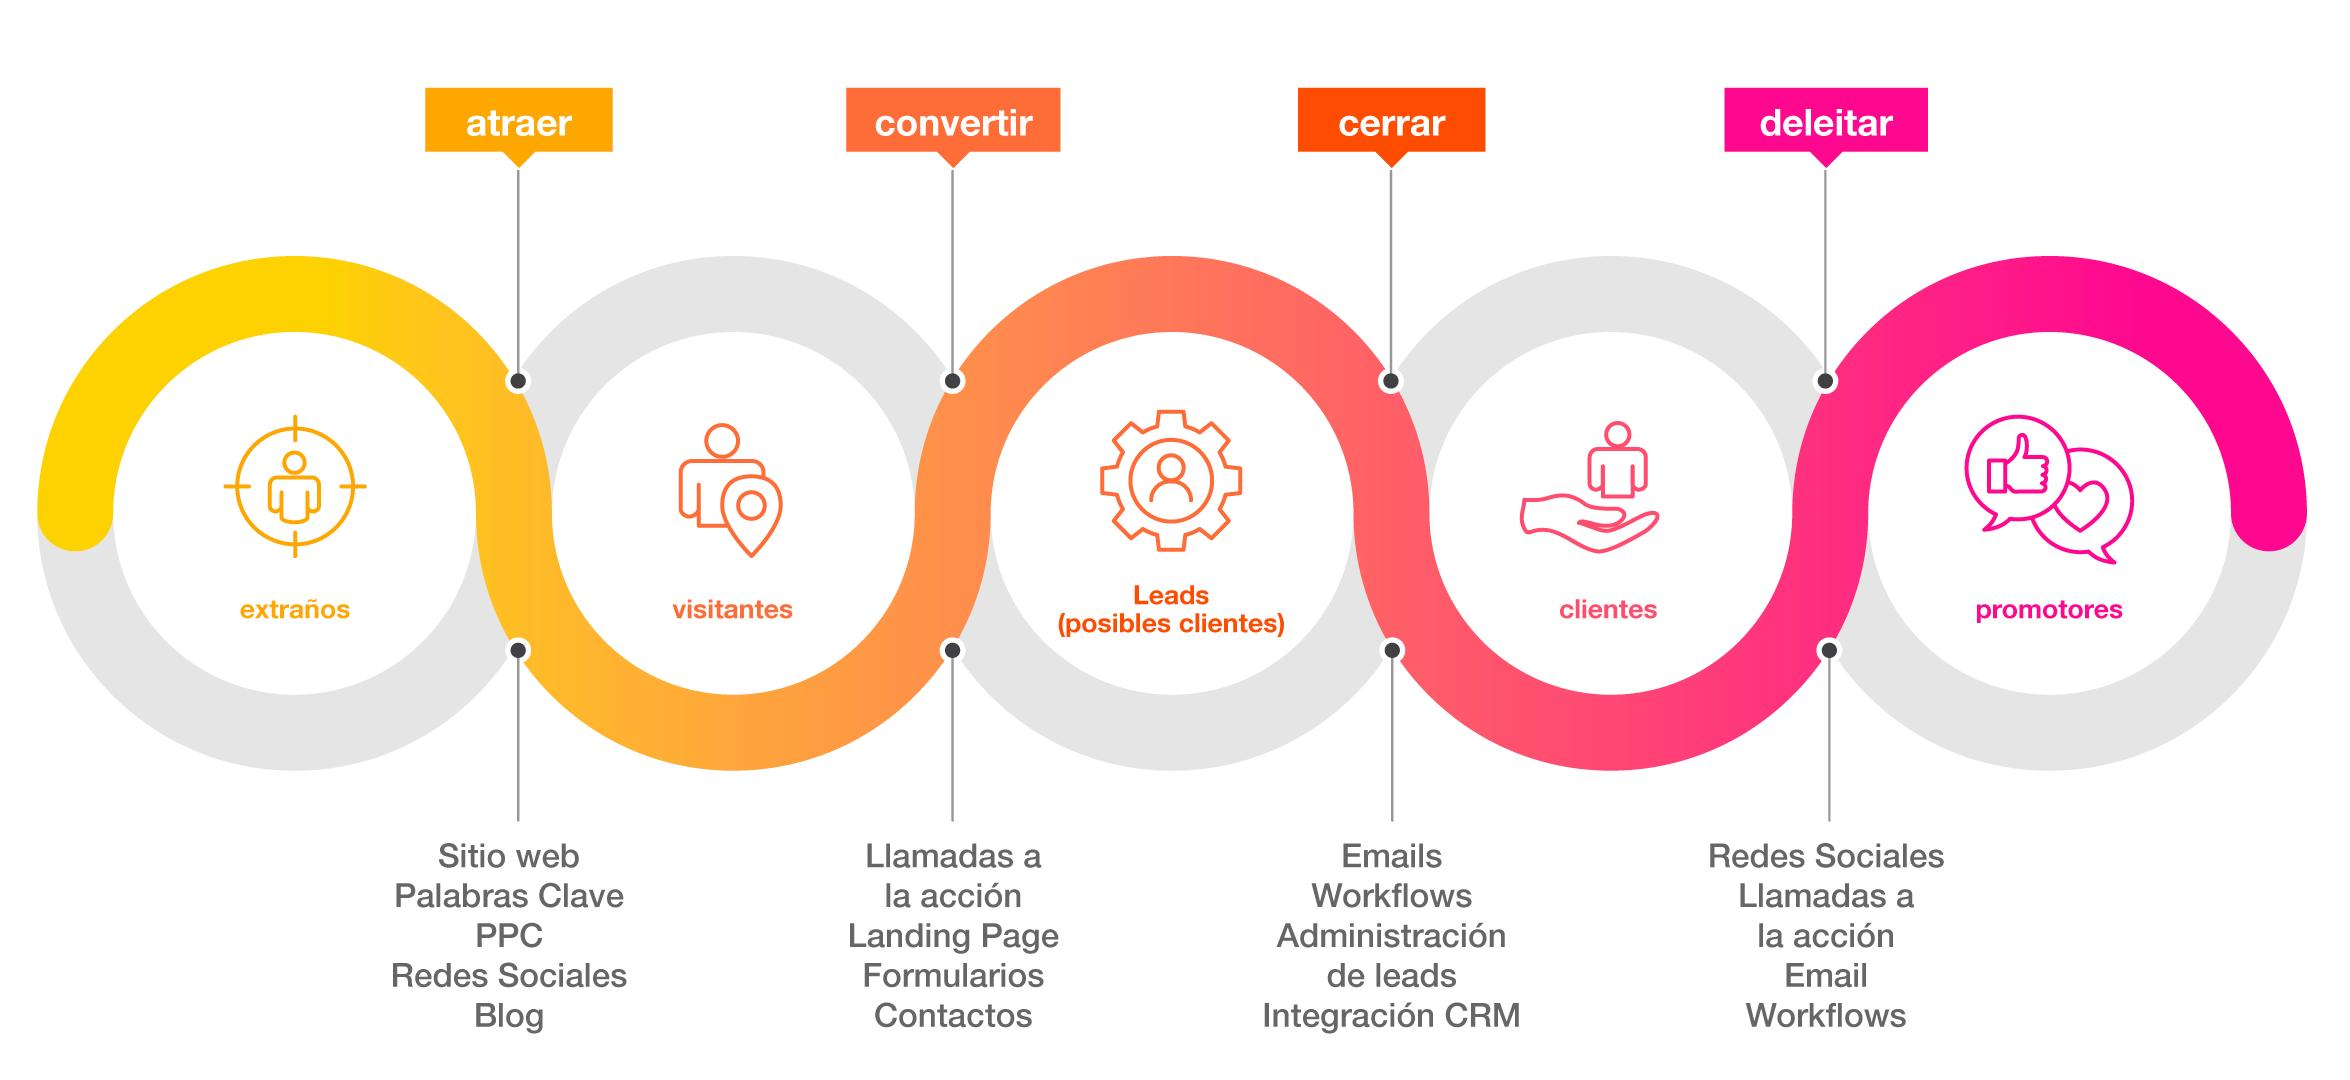
\includegraphics[width=0.8\textwidth]{Images/cms_inbound-marketingpng__YCPwBal20ZUUeH7LQ1Ze4XhRLfejrkRmN0YwTGOY.jpg}
          %esto es lo nuevo que agregue
        \fnote{Nota. \textup{Fuente: ¿Qué es Inbound Marketing?: Pasos para crear una estrategia efectiva (2019), \cite{de_2019}}}
\end{minipage}

Las 4 Fases de esta estrategias de marketing según Hubspot \cite{hubspot_2020} se pueden sintetizar como:

\begin{itemize}
    \item \textbf{Atraer: }Para generar tráfico, se deben emplear diferentes recursos como el marketing de contenidos, técnicas SEO, redes sociales, PPC, etc. Es importante que se haga de acuerdo con una planificación estratégica para conseguir resultados. El proyecto no se centrará en que una gran cantidad de usuarios visiten el sitio web, sino que se busca atraer a los usuarios que son potenciales compradores y clientes satisfechos. ¿Cómo hacerlo? Para llamar la atención de los clientes adecuados, se debe ofrecer contenido relevante en el momento adecuado.
    
    \item \textbf{Convertir:  }Una vez se logre captar la atención de los usuarios para que ingresen al sitio web, el siguiente paso es convertirlos en potenciales compradores. Para hacerlo, se debe iniciar una conversación de la manera que mejor se adapte a ellos; p. ej., a través de mensajes, formularios o reuniones.
    
    \item \textbf{Cerrar:  }Cerrar: Una vez que se tenga una base de datos, hay que gestionar los registros, integrarlos con un CRM (customer relationship management) o con herramientas de control y seguimiento.De esta manera, se crea un flujo de contenidos automatizado y adaptado al ciclo de compra del usuario; buscando determinar el momento adecuado para convertirlo en cliente.
    
    \item \textbf{Fidelizar:  }Cuando los usuarios pasen a formar parte del grupo de clientes de la organización, es necesario conservarlos. En esta fase, es necesario que perduren como clientes satisfechos, ofrecerles información útil e interesante y cuidar a tus posibles prescriptores para convertir las ventas en recomendaciones.
\end{itemize}


\subsubsection*{Precio}

Teniendo en cuenta el precio, variedad de servicios de reclutamiento personalizado y sus características de las soluciones ofrecidas por las diferentes empresas competidoras el precio de la Plataforma de Valoración Técnica de Profesionales TI usando Estrategias de Gamificación con Énfasis en Ingeniería Web se ha calculado teniendo en cuenta los siguientes factores:

\begin{itemize}
    \item Fidelización de clientes
    \item Optimización de los beneficios a corto y largo plazo
    \item Incursión eficaz y eficiente en el mercado
    \item Costos de mantención
    \item Producto similar en la competencia
    \item Demanda del servicio
    \item Soporte técnico
\end{itemize}
\begin{adjustbox}{
            center,
            caption=[{Precio en el mercado actual}]{\centering Precio en el mercado actual (Valores en pesos colombianos COP). },
            label={Precio},
            nofloat=table, vspace={20px}}
            {
            \begin{threeparttable}
           \begin{tabular}{|p{11cm}|p{10cm}p{2cm}|}
                \hline
                \rowcolor[HTML]{D9EAD3} 
                \cellcolor[HTML]{D9EAD3}                              & \multicolumn{2}{c|}{\cellcolor[HTML]{D9EAD3}Precio}            \\ \cline{2-3} 
                \rowcolor[HTML]{D9EAD3} 
                \multirow{-2}{*}{\cellcolor[HTML]{D9EAD3}Suscripción} & \multicolumn{1}{l|}{\cellcolor[HTML]{D9EAD3}Mínimo} & Máximo   \\ \hline
                \multicolumn{1}{|l|}{Mensualidad}                     & \multicolumn{1}{l|}{\$170000}                       & \$530000 \\ \hline
            \end{tabular}
            \begin{tablenotes}[para,flushleft]
                \vspace{2mm}
               \textit Nota. Fuente: : Autores.
            \end{tablenotes}
            
        \end{threeparttable} 
    }        
            
\end{adjustbox}

Si bien los precios que existen actualmente en el mercado son bastante competitivos y sus modelos de negocio muy similares, el factor diferencial que resalta en el proyecto viene por su bajo precio de subscripción mensual y en el cobro por comisión por aspirantes con pruebas exitosas, la cual proporciona la mayor cantidad de ingresos. Nuestro modelo de negocios contara tanto con un servicio de suscripción por periodos:


\begin{adjustbox}{
            center,
            caption=[{Precios de suscripción.}]{Precios de suscripción mensual, trimestral y anual. },
            label={PrecioPeriodos},
            nofloat=table, vspace={20px}}
            {
            \begin{threeparttable}
           \begin{tabular}{|p{7.8cm}|p{7.8cm}|}
            \hline
            \rowcolor[HTML]{D9EAD3} 
            Suscripción & Precio       \\ \hline
            Mensualidad & \$ 90.000    \\ \hline
            Trimestre   & \$ 250.000   \\ \hline
            Anualidad   & \$ 1.000.000 \\ \hline
            \end{tabular}%
            
            \begin{tablenotes}[para,flushleft]
                \vspace{2mm}
                \textit Nota. Fuente: : Autores.
            \end{tablenotes}
            
        \end{threeparttable} 
    }        
            
\end{adjustbox}